\documentclass[12pt]{article}
\usepackage{amsmath}
\usepackage{graphicx}
\usepackage{hyperref}
\usepackage{listings}
\usepackage{color}
\usepackage{pythonhighlight}

\title{Operating System Course Report - First Half of the Semester}
\author{A class}
\date{\today}

\begin{document}

\maketitle
\newpage

\tableofcontents
\newpage

\section{Introduction}
This report summarizes the topics covered during the first half of the Operating System course. It includes theoretical concepts, practical implementations, and assignments. The course focuses on the fundamentals of operating systems, including system architecture, process management, CPU scheduling, and deadlock handling.

\section{Course Overview}
\subsection{Objectives}
The main objectives of this course are:
\begin{itemize}
    \item To understand the basic components and architecture of a computer system.
    \item To learn process management, scheduling, and inter-process communication.
    \item To explore file systems, input/output management, and virtualization.
    \item To study the prevention and handling of deadlocks in operating systems.
\end{itemize}

\subsection{Course Structure}
The course is divided into two halves. This report focuses on the first half, which covers:
\begin{itemize}
    \item Basic Concepts and Components of Computer Systems
    \item System Performance and Metrics
    \item System Architecture of Computer Systems
    \item Process Description and Control
    \item Scheduling Algorithms
    \item Process Creation and Termination
    \item Introduction to Threads
    \item File Systems
    \item Input and Output Management
    \item Deadlock Introduction and Prevention
    \item User Interface Management
    \item Virtualization in Operating Systems
\end{itemize}

\section{Topics Covered}

\subsection{Basic Concepts and Components of Computer Systems}
This section explains the fundamental components that make up a computer system, including the CPU, memory, storage, and input/output devices.

\subsection{Performa Sistem dan Metrik Sistem Komputer}
\subsubsection{Performa Sistem}
Performa sistem komputer adalah kemampuan suatu sistem untuk menjalankan tugas-tugas komputasi sesuai dengan spesifikasi dan parameter yang telah ditetapkan. Performa ini mencakup kecepatan, efisiensi, dan ketepatan dalam menyelesaikan berbagai proses dan operasi yang diminta oleh pengguna atau aplikasi.
\begin{enumerate}
    \item {Faktor Pengaruh Peforma}
    \par \begin{enumerate}
        \item {CPU (Central Processing Unit)}
        \par CPU atau prosesor adalah otak dari komputer yang bertanggung jawab untuk menjalankan instruksi dan menjalankan proses komputasi. Kecepatan CPU diukur dalam gigahertz (GHz), dan semakin tinggi frekuensi, semakin cepat proses eksekusi instruksi. Selain itu, jumlah core pada CPU juga memainkan peran penting; semakin banyak core, semakin baik komputer dalam menangani multitasking dan menjalankan aplikasi yang membutuhkan banyak sumber daya.
        \item {GPU (Graphics Processing Unit)}
        \par GPU bertanggung jawab untuk menangani pemrosesan grafis dan rendering visual. Dalam aplikasi yang membutuhkan performa grafis tinggi seperti game, desain 3D, atau pengeditan video, GPU yang kuat menjadi sangat penting. GPU modern juga digunakan untuk komputasi paralel di bidang kecerdasan buatan dan pembelajaran mesin, mempercepat proses yang tidak bisa ditangani dengan efisien oleh CPU.
        
        \item {RAM (Random Access Memory)}
        \par RAM adalah memori sementara yang digunakan oleh sistem untuk menyimpan data yang aktif digunakan atau diakses oleh CPU dengan cepat. Kapasitas RAM yang lebih besar memungkinkan komputer untuk menjalankan lebih banyak aplikasi secara bersamaan atau memproses data yang lebih besar tanpa memperlambat performa. Selain itu, kecepatan RAM juga berpengaruh pada seberapa cepat data dapat diakses dan diproses.

        \item {Penyimpanan (Storage)}
        \par Jenis dan kapasitas penyimpanan berperan besar dalam kecepatan akses data. Penyimpanan berbasis SSD (Solid State Drive) jauh lebih cepat dibandingkan dengan HDD (Hard Disk Drive) tradisional, yang memungkinkan komputer untuk memuat program dan mengakses file dengan lebih cepat. SSD meningkatkan performa keseluruhan sistem, terutama dalam hal waktu boot, pembukaan aplikasi, dan kecepatan transfer file.

    \end{enumerate}
    \item {Keterkaitan Hardware}
    \par \begin{enumerate}
        \item {{Keterkaitan antara RAM dan CPU}}
        \par CPU bergantung pada RAM untuk menyimpan data sementara yang sedang diproses. Ketika CPU menjalankan tugas, ia membutuhkan data yang dapat diakses dengan cepat. RAM menyediakan ruang penyimpanan sementara yang memungkinkan CPU untuk mengakses data dengan kecepatan tinggi, yang membantu mencegah penundaan dalam pemrosesan. Semakin besar kapasitas dan kecepatan RAM, semakin cepat CPU dapat memproses data, terutama dalam situasi multitasking di mana banyak aplikasi berjalan secara bersamaan.
    
        \item {{Keterkaitan antara CPU dan GPU}}
        \par CPU dan GPU bekerja bersama-sama untuk membagi tugas yang memerlukan pemrosesan berat. CPU menangani tugas-tugas umum seperti logika, kontrol aplikasi, dan aliran data, sementara GPU menangani tugas-tugas yang membutuhkan komputasi paralel, seperti rendering grafis atau komputasi numerik. Kinerja keseluruhan sistem meningkat ketika CPU dan GPU dapat bekerja secara seimbang. Jika salah satu komponen terlalu lambat dibandingkan dengan yang lain, bisa terjadi bottleneck, di mana salah satu perangkat keras menahan kinerja perangkat lainnya.
    
        \item {{Keterkaitan antara Penyimpanan dan RAM}}
        \par RAM dan penyimpanan juga bekerja sama untuk memastikan kelancaran operasi sistem. Ketika aplikasi atau data yang dibutuhkan oleh CPU tidak dapat seluruhnya ditampung di RAM, sistem akan menggunakan penyimpanan sebagai memori virtual. Jika penyimpanan yang digunakan adalah SSD (Solid State Drive), maka akses data dari penyimpanan ke RAM menjadi jauh lebih cepat dibandingkan dengan HDD (Hard Disk Drive) tradisional, sehingga mempercepat pemuatan aplikasi dan respons sistem secara keseluruhan.
    
    \end{enumerate} 

\end{enumerate}
    


\subsubsection{Metrik Sistem Utama}
\begin{enumerate}
    \item Throughput
\end{enumerate}

Throughput adalah jumlah output yang dapat diselesaikan oleh sistem dalam jangka waktu tertentu, misalnya jumlah permintaan yang dilayani oleh server dalam satu detik. Contoh Kasus: Server Web: Sebuah server web yang mampu melayani 200 permintaan HTTP per detik memiliki throughput sebesar 200 request per second. Jika throughput rendah, server mungkin membutuhkan peningkatan kapasitas. Optimasi: Throughput dapat ditingkatkan dengan mempercepat prosesor atau meningkatkan bandwidth jaringan untuk menangani lebih banyak permintaan secara simultan. 

 2.Latency
Definisi: Latency adalah waktu yang diperlukan untuk menyelesaikan satu unit kerja dari awal hingga akhir, misalnya waktu tunggu antara saat data dikirim dan diterima. Contoh Kasus: Sistem Jaringan: Dalam jaringan, jika waktu yang dibutuhkan untuk mengirim paket data dari satu komputer ke komputer lain adalah 20 milidetik, ini mencerminkan tingkat latency. Latency yang tinggi dapat menyebabkan keterlambatan dalam komunikasi, yang dapat mengganggu aplikasi seperti video conference. Optimasi: Latency dapat dikurangi dengan menggunakan jalur komunikasi yang lebih cepat atau memperbaiki routing jaringan untuk menghindari keterlambatan.

 Utilization
Definisi: Utilization mengukur tingkat penggunaan sumber daya
sistem, seperti CPU atau memori, dan biasanya dinyatakan
dalam persentase.
Contoh:
Server Database: Jika sebuah server database menunjukkan
CPU utilization sebesar 90%, ini menandakan bahwa CPU bekerja
sangat keras, yang bisa menjadi tanda overutilization.
Overutilization dapat menyebabkan penurunan performa
keseluruhan sistem.
Optimasi: Utilization dapat dikurangi dengan menambahkan lebih
banyak CPU, menyeimbangkan beban kerja di antara server
lain, atau mengoptimalkan kode aplikasi untuk efisiensi yang
lebih tinggi.

 Response time
Definisi: Response time adalah waktu yang diperlukan oleh sistem untuk merespons permintaan dari pengguna, misalnya waktu yang diperlukan untuk memproses pembayaran dalam aplikasi e-commerce.


\subsubsection{Metrik Sistem Spesifik}
\begin{enumerate}
    \item Cycle Per Instruction (CPI)
    \par CPI adalah salah satu metrik utama yang digunakan untuk mengevaluasi performa CPU (Central Processing Unit). CPI mengukur rata-rata jumlah siklus clock yang dibutuhkan oleh CPU untuk mengeksekusi satu instruksi.
    \par Formula umum CPI: 
    \par CPI = Total Cycle Total/Instructions
    \par Rendahnya CPI berarti CPU dapat mengeksekusi instruksi lebih efisien, menunjukkan performa yang lebih baik sedangkan tingginya CPI menunjukkan bahwa CPU memerlukan lebih banyak siklus clock untuk mengeksekusi instruksi, yang bisa berarti instruksi tersebut lebih kompleks ata ada masalah dalam pipeline CPU.
    \par Contoh Penggunaan CPI
    \par Misalkan kamu memiliki dua CPU: 
    \par CPU A memiliki CPI 1.2 
    \par CPU B memiliki CPI 1.8 
    \par Jika keduanya berjalan pada frekuensi yang sama, katakanlah 3 GHz, CPU A akan lebih efisien karena membutuhkan lebih sedikit siklus per instruksi. Ini berarti CPU A dapat menyelesaikan lebih banyak instruksi dalam waktu yang sama dibandingkan CPU B.

    \item Floating Point Operations Per Second (FLOPS)
    \par FLOPS adalah metrik yang digunakan untuk mengukur
    kemampuan komputasi floating-point dari sebuah
    komputer, yang sangat penting dalam aplikasi yang
    memerlukan kalkulasi numerik berat, seperti simulasi
    ilmiah, pemodelan 3D, atau machine learning.
    \par Contoh Penggunaan FLOPS:
    \par Bayangkan kamu bekerja di bidang simulasi ilmiah yang memerlukan perhitungan numerik yang intensif. Sistem A memiliki kapasitas 2 TFLOPS, sementara Sistem B memiliki 5 TFLOPS. Sistem B akan mampu menyelesaikan simulasi tersebut lebih cepat, karena dapat melakukan lebih banyak operasi floating-point per detik.

    \item Input/Output Operations Per Second (IOPS)
    \par IOPS mengukur performa dari perangkat penyimpanan (seperti SSD, HDD) dalam hal jumlah operasi input/output yang dapat diproses dalam satu detik. IOPS sering digunakan untuk mengevaluasi performa disk dan sistem penyimpanan.
    \par Contoh Penggunaan IOPS:
    \par Misalkan kamu mengelola server database. SSD A memiliki 100,000 IOPS, sementara SSD B memiliki 50,000 IOPS. SSD A akan mampu menangani lebih banyak operasi baca/tulis per detik, sehingga lebih cocok untuk lingkungan database yang memerlukan akses data cepat dan simultan.
    
\end{enumerate}



\subsubsection{Pengukuran dan Optimasi Performa}
\begin{enumerate}
    \item {Pengukuran performa}
    \par Pengukuran performa mengacu pada proses mengukur sejauh mana suatu sistem, aplikasi, atau proses memenuhi tujuan performa yang telah ditentukan. Hal ini sangat penting karena memberikan gambaran yang jelas mengenai efektivitas, efisiensi, dan kualitas suatu sistem atau aplikasi.
    \begin{enumerate}
        \item Benchmarking
        \par Benchmarking adalah metode pengujian serangkaian program dengan cara membandingkan performa suatu sistem terhadap performa standar untuk mendapatkan performa relatif dari komponen PC atau sistem. Tujuan dari benchmarking adalah untuk memberikan gambaran yang jelas tentang performa sistem komputer sehingga dapat dipastikan bahwa teknologi atau perangkat yang digunakan optimal dan memenuhi standar industri. Ada 2 jenis dari benchmarking:
        \begin{itemize}
        \item Synthetic benchmarking: Simulasi skenario tertentu untuk mengukur potensi maksimum performa sistem, seperti menggunakan SPEC CPU untuk menguji kemampuan komputasi CPU.
        \item Real-world Benchmarking: Pengukuran performa sistem menggunakan aplikasi nyata dalam kondisi operasional sehari-hari, seperti Adobe Premiere Pro untuk menguji kecepatan rendering video.
    \end{itemize}  
    \item Profiling
    \par Profiling adalah metode untuk menganalisis performa aplikasi atau sistem secara mendalam dengan fokus pada penggunaan sumber daya internal. Profiling membantu mengidentifikasi bagian dari sistem atau program yang mengkonsumsi sumber daya paling banyak, seperti CPU, memori, I/O, dan waktu eksekusi. Dengan demikian, profiling digunakan untuk menemukan dan memperbaiki "bottleneck" dalam aplikasi atau sistem, memungkinkan pengembang untuk melakukan optimasi yang tepat. Berikut beberapa metode dalam profiling:
    \begin{itemize}
        \item CPU Profiling: Mengukur penggunaan CPU untuk mengidentifikasi kode yang paling memakan waktu. \textit{Tools} yang digunakan yaitu gprof dan Perf.
        \item Memory Profiling: Mengukur alokasi memori dan menemukan kebocoran memori. \textit{Tools} yang digunakan yaitu Valgrind dan Heap Profiler.
        \item I/O Profiling: Menganalisis performa operasi input/output seperti file atau jaringan. \textit{Tools} yang digunakan yaitu IOTop dan dstat.
        \item Function-Level Profiling: Menganalisis fungsi dalam aplikasi, melihat frekuensi pemanggilan dan durasi. \textit{Tools} yang digunakan yaitu Xdebug (PHP) dan py-spy (Python).
    \end{itemize}
    \item Monitoring
    \par Monitoring adalah proses pengamatan dan pengukuran performa sistem secara real-time dan berkelanjutan untuk memastikan sistem berjalan optimal serta mendeteksi masalah atau potensi gangguan. Monitoring sangat penting untuk menjaga stabilitas dan performa sistem komputer atau aplikasi, terutama dalam lingkungan produksi, di mana uptime dan keandalan menjadi prioritas. Ada beberapa teknik yang sering digunakan dalam monitoring:
    \begin{itemize}
        \item Real-Time monitoring:
        \par Memantau sistem secara langsung dan memberikan informasi performa atau kegagalan segera setelah terjadi. Real-time monitoring sangat penting untuk aplikasi dengan kebutuhan uptime tinggi, seperti layanan berbasis cloud, sistem e-commerce, atau server.
        \item Historical Monitoring:
        \par Mengumpulkan data performa selama jangka waktu tertentu dan menyimpannya untuk dianalisis kemudian. Ini penting untuk analisis tren dan perencanaan kapasitas, karena memungkinkan tim IT untuk melihat bagaimana sistem telah beroperasi dalam jangka waktu tertentu.
        \item Threshold-Based Monitoring:
        \par Sistem monitoring yang memberikan notifikasi atau alarm ketika nilai performa melebihi atau di bawah batas tertentu. Misalnya, jika penggunaan CPU melebihi 90\% atau penggunaan memori terlalu rendah, sistem akan mengirimkan peringatan kepada administrator.
    \end{itemize}
    \begin{table}[htbp]
    \centering
        \begin{tabular}{|p{2cm}|p{3cm}|p{3cm}|p{3cm}|}
        \hline
        Aspek & Benchmarking & Profiling & Monitoring \\
        \hline
        Fokus & Performa keseluruhan terhadap standar & Analisis mendalam per bagian sistem & Pemantauan performa real-time \\
        \hline
        Tujuan & Perbandingan performa & Optimasi performa & Menjaga kestabilan sistem \\
        \hline
        Dilakukan saat & Di bawah kondisi spesifik (uji beban) & Saat pengembangan atau testing & Selama sistem berjalan (operasional) \\
        \hline
        Hasil utama & Angka perbandingan & Identifikasi \textit{bottleneck} & Data penggunaan sumber daya \\
        \hline
        \end{tabular}
        \caption{Perbedaan dari Benchmarking, Profiling, dan Monitoring}
        \label{table:ringkasan_perbedaan}
    \end{table}
    \end{enumerate}
    \item {Strategi Optimasi Performa}
    \par 
\end{enumerate}



\subsection{System Architecture of Computer Systems}
Describes the architecture of modern computer systems, focusing on the interaction between hardware and the operating system.

\subsection{Process Description and Control}
Processes are a central concept in operating systems. This section covers:
\begin{itemize}
    \item Process states and state transitions
    \item Process control block (PCB)
    \item Context switching
\end{itemize}

\subsection{Scheduling Algorithms}
This section covers:
\begin{itemize}
    \item First-Come, First-Served (FCFS)
    \item Shortest Job Next (SJN)
    \item Round Robin (RR)
\end{itemize}
It explains how these algorithms are used to allocate CPU time to processes.

\subsection{Process Creation and Termination}
Details how processes are created and terminated by the operating system, including:
\begin{itemize}
    \item Process spawning
    \item Process termination conditions
\end{itemize}

\subsection{Introduction to Threads}
This section introduces the concept of threads and their relation to processes, covering:
\begin{itemize}
    \item Single-threaded vs. multi-threaded processes
    \item Benefits of multithreading
\end{itemize}

\begin{figure}[h]
    \centering
    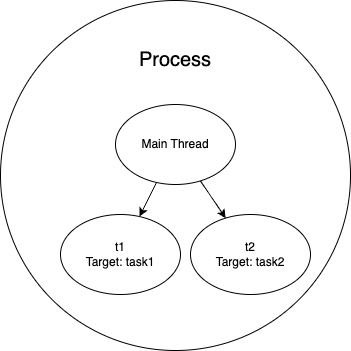
\includegraphics[width=0.5\textwidth]{/Users/khawaritzmi/Unhas/os_report_mid2024/a_class/asset/example.png}  % Sesuaikan nama file dan ukurannya
    \caption{Ini adalah gambar contoh dari multithreading.}
    \label{fig:contoh_gambar}
\end{figure}

Seperti yang terlihat pada Gambar \ref{fig:contoh_gambar}, inilah cara menambahkan gambar dengan keterangan.

\subsection{File Systems}
File systems provide a way for the operating system to store, retrieve, and manage data. This section explains:
\begin{itemize}
    \item File system structure
    \item File access methods
    \item Directory management
\end{itemize}

\subsection{Input and Output Management}
Input and output management is key for handling the interaction between the system and external devices. This section includes:
\begin{itemize}
    \item Device drivers
    \item I/O scheduling
\end{itemize}

\subsection{Deadlock Introduction and Prevention}
Explores the concept of deadlocks and methods for preventing them:
\begin{itemize}
    \item Deadlock conditions
    \item Deadlock prevention techniques
\end{itemize}

\subsection{User Interface Management}
This section discusses the role of the operating system in managing the user interface. Topics covered include:
\begin{itemize}
    \item Graphical User Interface (GUI)
    \item Command-Line Interface (CLI)
    \item Interaction between the user and the operating system
\end{itemize}

\subsection{Virtualization in Operating Systems}
Virtualization allows multiple operating systems to run concurrently on a single physical machine. This section explores:
\begin{itemize}
    \item Concept of virtualization
    \item Hypervisors and their types
    \item Benefits of virtualization in modern computing
\end{itemize}

\section{Assignments and Practical Work}
\subsection{Assignment 1: Process Scheduling}
Students were tasked with implementing various process scheduling algorithms (e.g., FCFS, SJN, and RR) and comparing their performance under different conditions.
\subsubsection{Group 1}
\begin{python}
    class Process:
    def __init__(self, pid, arrival_time, burst_time):
        self.pid = pid
        self.arrival_time = arrival_time
        self.burst_time = burst_time
        self.completion_time = 0
        self.turnaround_time = 0
        self.waiting_time = 0
\end{python}

\begin{table}[htbp] % Optional: For floating position
    \centering
    \begin{tabular}{|c|c|c|} % Defines number of columns and alignment (c = center, l = left, r = right). '|' creates vertical lines.
    \hline
    Header 1 & Header 2 & Header 3 \\ % Column headers
    \hline
    Row 1, Column 1 & Row 1, Column 2 & Row 1, Column 3 \\ % First row of data
    \hline
    Row 2, Column 1 & Row 2, Column 2 & Row 2, Column 3 \\ % Second row of data
    \hline
    \end{tabular}
    \caption{Your table caption} % Optional: For adding a caption
    \label{tab:your_label} % Optional: For cross-referencing the table
\end{table}
\subsection{Assignment 2: Deadlock Handling}
In this assignment, students were asked to simulate different deadlock scenarios and explore various prevention methods.

\subsection{Assignment 3: Multithreading and Amdahl's Law}
This assignment involved designing a multithreading scenario to solve a computationally intensive problem. Students then applied **Amdahl's Law** to calculate the theoretical speedup of the program as the number of threads increased.

\subsection{Assignment 4: Simple Command-Line Interface (CLI) for User Interface Management}
Students were tasked with creating a simple **CLI** for user interface management. The CLI should support basic commands such as file manipulation (creating, listing, and deleting files), process management, and system status reporting.

\subsection{Assignment 5: File System Access}
In this assignment, students implemented file system access routines, including:
\begin{itemize}
    \item File creation and deletion
    \item Reading from and writing to files
    \item Navigating directories and managing file permissions
\end{itemize}

\section{Conclusion}
The first half of the course introduced core operating system concepts, including process management, scheduling, multithreading, and file system access. These topics provided a foundation for more advanced topics to be covered in the second half of the course.

\end{document}